\documentclass[11pt]{article}
\usepackage[utf8]{inputenc}
\usepackage{amsmath}
\usepackage{amssymb}
\usepackage{graphicx}
\usepackage{hyperref}
\usepackage[parfill]{parskip}
\let\oldemptyset\emptyset
\let\emptyset\varnothing


\title{\textbf{Esssentials of Applied Data Analysis\\
				IPSA-USP Summer School 2017}\newline\\
				Introduction to Random Variables}

\author{Leonardo Sangali Barone\\ \href{leonardo.barone@usp.br}{leonardo.barone@usp.br}}
\date{jan/17}

\begin{document}

\maketitle

\section*{Random Variables}

	\subsection*{Theory, Concepts and Variables}

	\begin{itemize}

	\item A theory is a set of statements that involve concepts.
	\item Concepts are inventions that help us understand the world.
	\item Theories (and the hypotheses they imply) concern relationships among abstract concepts.
	\end{itemize}
	What is a variable? A variable is simply an indicator we develop to measure our concepts.


	\subsection*{Variables \emph{versus} constants}
	A constant is a variable that can assume only one value. For example: if we want to use survey data of women teenagers to compute abortion rates, sex of the subjects is not a variable, is a constant\\
	
	Golden rule: a variable must vary!

	\subsection*{Types of Variables}
	
	A) Discrete - values are countable, even if infinite.
	
	\begin{itemize}
		\item Nominal - can be counted, but not ordered
		\item Ordinal - can be counted and ordered
		\item Integer - can be counted, ordered and the distance between categories are mathematically meaningful (yes, numbers with no decimals).
	\end{itemize}
	
	B) Continuous - Infinite set of values. Not countable (yes, whatever number there is, including $\sqrt{2} $ and $\pi$). \\

	Can you think of some examples of each type of variable?\\

	Whatch out! Nominal and Ordinal variable's categories can be coded with numbers, but mathematical operations with those numbers are not possible (if it were, they would be Integer variables).

\section*{Random variables, distributions and probability functions}

	\emph{Probability function} is a function that describes the likelihood of the values a concept (variable) might take given a description of the process that generates it.\\
	
	What?!?!?!?\\

	We have already studied the rules of probability. Now, we are going to use our knowledge of probability to learn about random variables.\\
	
	A \emph{probability function} is just a function that indicates the probability of each value (events!!!) of a random variable (measurements of concepts!!!). We usually represent it as any other function, $f(x)$, and it is defined as:
	
	\[f(x) = P(X=x)\]
	
	One way to think about it is that it is a mapping function, since it "maps" the probability associated with each value of a random variable ($X$).\\	

\begin{figure}[htp]
\centering
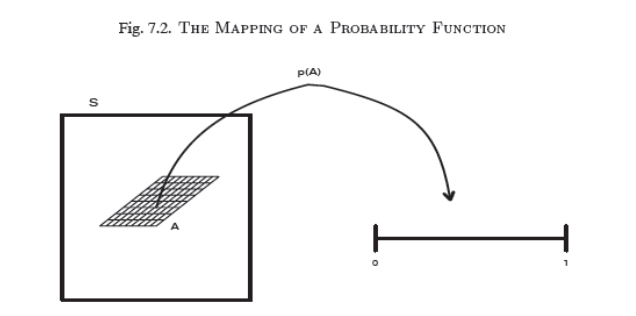
\includegraphics[scale=0.70]{mapping.png}
\caption{Mapping function}
\label{}
\end{figure}	

	\emph{Random variable} doesn't mean we are picking any variable randomly,	but a variable that can take some array of values, with the probability that it takes any particular value defined according to some random process.\\

	The set of values the variable might take is the  \emph{distribution} of the random variable.\\

	The probability function gives us the probability distribution of a random variable. Conventionally, we call it \emph{probability mass function} if the variable is discrete and \emph{probability density function} if the variable is continuous.

	Some random variables in political science:
	
	\begin{itemize}
		\item Voter's choice
		\item Government regimes; electoral systems
		\item Choices of policy and policy paths
		\item \% of votes in an election
		\item Number of parties in a cabinet
		\item Time past since the last war/disaster
		\item Public health care system expenditure
		\item Number of families/individuals in a program
	\end{itemize}
	Can you think of some more?


\end{document}
